\documentclass[11pt]{article}
\usepackage[top=1cm, bottom=2cm, left=1cm, right=1cm]{geometry}
\usepackage{ctex}
\usepackage{algorithm}
\usepackage{algorithmicx}
\usepackage{algpseudocode}
\usepackage{amsthm,amsmath,amssymb}
\usepackage[colorlinks=true,linkcolor=blue]{hyperref}
\usepackage{listings}
\usepackage{xcolor,xparse}
\usepackage{realboxes}
\usepackage{graphics}
\usepackage{graphicx}
\usepackage{mathrsfs}
\usepackage{wrapfig}
\usepackage{subfigure}
\usepackage{pifont}

\definecolor{cmdbg}{rgb}{0.9,0.9,0.9}
\lstset{%
	basicstyle=\ttfamily,
	breaklines = true,
	backgroundcolor=\color{cmdbg},
}
\DeclareDocumentCommand{\ccmd}{v}{% 参数 v 表示工作方法类似于 \verb
    \Colorbox{cmdbg}{\csname lstinline\endcsname!#1!}%
}

\makeatletter
\newenvironment{breakablealgorithm}
  {% \begin{breakablealgorithm}
   \begin{center}
     \refstepcounter{algorithm}% New algorithm
     \hrule height.8pt depth0pt \kern2pt% \@fs@pre for \@fs@ruled
     \renewcommand{\caption}[2][\relax]{% Make a new \caption
       {\raggedright\textbf{\ALG@name~\thealgorithm} ##2\par}%
       \ifx\relax##1\relax % #1 is \relax
         \addcontentsline{loa}{algorithm}{\protect\numberline{\thealgorithm}##2}%
       \else % #1 is not \relax
         \addcontentsline{loa}{algorithm}{\protect\numberline{\thealgorithm}##1}%
       \fi
       \kern2pt\hrule\kern2pt
     }
  }{% \end{breakablealgorithm}
     \kern2pt\hrule\relax% \@fs@post for \@fs@ruled
   \end{center}
  }
\makeatother

\author{李明钰 22307110156}
\title{计算物理作业2}

\begin{document}
\maketitle

\section{题目1:画函数图像$x^3-5x+3=0$}
首先,我们画出大致的函数图像如图\ref{fig:第一问函数图像的大致形状}所示,容易观察到,其有两个正根,分别处于(0,1)和(1,2)上。
\begin{figure}
    \centering
    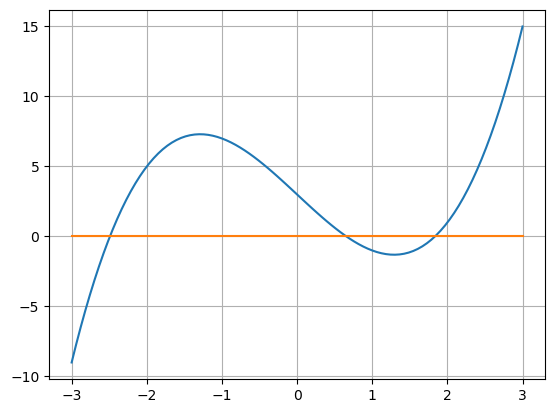
\includegraphics[width=0.5\textwidth]{第一问函数图像的大致形状.png}
    \caption{第一问函数图像的大致形状}
    \label{fig:第一问函数图像的大致形状}
\end{figure}

\subsection{第一问:用二分法将两个正根精确到小数点后四位}
\subsubsection{程序描述}
题目要求使用二分法求根,选择最初的区间长度为1,$2^{14}=16384$,只需迭代14次即可达到要求。利用算法\ref{Bisection method},设置函数为$f(x)=x^3-5x+3=0$,区间分别为(0,1)和(1,2)并设置$n=14$即可达到所需效果。

\subsubsection{伪代码}
\begin{breakablealgorithm}    
    \caption{Bisection method}
    \label{Bisection method}
    \begin{algorithmic}
        \Require $a,b$ :float \quad $n$:int \quad $f$:function
        \Ensure root
        \State $x_{l,0} = a  \quad x_{r,0}=b x_0 = \frac{x_{l,0}+x_{r,0}}{2} \quad$
        \For{$k \gets 0$ \textbf{to} n}
        \If{$f(x)\times f(x_{l,k})<0$}
        \State $x_{l,(k+1)}=x_{l,k}\quad x_{r,(k+1)}=x_k$
        \Else 
        \State $x_{l,(k+1)}=x_{k}\quad x_{r,(k+1)}=x_{r,k}$
        \EndIf
        $x_{(k+1)} = \frac{x_{l,(k+1)+x_{r,(k+1)}}+}{2}$
        \EndFor
        \State\Return $x_n$
    \end{algorithmic}
\end{breakablealgorithm}

\subsubsection{输出实例}
如图\ref{fig:第一问输出实例}所示。
\begin{figure}
    \centering
    
\includegraphics[width=0.5\textwidth]{第一问输出实例.png}
    \caption{第一问输出实例}
    \label{fig:第一问输出实例}
\end{figure}
\subsection{第二问:在第一问基础上用牛顿法将小数点精确到14位}
先计算出其导数,记为$g(x) = \frac{df}{dx} = 3x^2-5$
\subsubsection{程序描述}
由第一问所求出的零点的大致位置,可以得到,在零点位置处的导数约为-3.7和5.1,通过估算和实际尝试,用牛顿法(算法\ref{Newton-Raphson Method})迭代约20次(n取20)的情况下,解将收敛且精度达到14位小数。
\subsubsection{伪代码}
\begin{breakablealgorithm}
    \caption{Newton-Raphson Method}
    \label{Newton-Raphson Method}
    \begin{algorithmic}
        \Require $x_0$:float \quad n:int \quad $f$:function 
        \Ensure $root$
        \State $g = f'$
        \For{$k \gets 1 \textbf{ to } n$}
        \State$x_{(k+1)} = x-\frac{f(x_k)}{g(x_k)}$
        \EndFor
        \State \Return $x_n$
    \end{algorithmic}
\end{breakablealgorithm}

\subsubsection{输出实例}
如图\ref{fig:第二问输出实例}所示
\begin{figure}
    \centering
    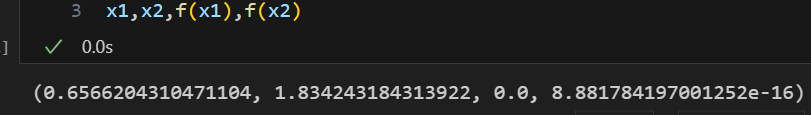
\includegraphics[width=0.5\textwidth]{第二问输出实例.png}
    \caption{第二问输出实例}
    \label{fig:第二问输出实例}
\end{figure}

\subsection{第三问:用混合方法计算根至小数点后14位}
\subsection{程序描述}
从收敛性角度来看,二分法是线性收敛而牛顿法是二次收敛,因此牛顿法更好,但是牛顿法有一个致命缺点,当迭代过程中出现某一$x_k$使得$\frac{df}{dx}|_{x_k} = 0$时,将无法继续迭代,因此,采用与二分法相结合的方式,在牛顿法无法迭代时,采用二分法进行迭代,即算法
在本题目中,不再人为限定迭代次数,而是设置为持续迭代至$|{f(x_k)|<\epsilon}$时认为其已经收敛,因为主要还是靠牛顿法进行迭代,由第二问所算出的在根附近f的导数值,认为设$\epsilon=10^{-15}$即可达到所要求的精度。
\subsubsection{伪代码}
\begin{breakablealgorithm}
    \caption{Newton Bisection Hybrid}
    \label{Newton Bisection Hybrid}
    \begin{algorithmic}
        \Require $(a,b):float \quad \epsilon:float \quad f:function$
        \Ensure root
        \State $x_0 = \frac{a+b}{2}\quad x_{l}=a \quad x_{r} = b \quad g(x) = \frac{df}{dx}$
        \While {$|f(x)|>\epsilon$}
            \If {$g(x_r)=0$}
                \If{$f(x_l)\cdot f(x_0)<0$}
                \State $x_l \gets x_l \quad x_r \gets x_0 \quad x_0 \gets \frac{x_l+x_r}{2}$      
                \Else
                \State $x_l \gets x_0 \quad x_r \gets x_r \quad x_0 \gets \frac{x_l+x_r}{2}$
                \EndIf
            \Else
            \State $x_{0} \gets x_0-\frac{f(x_0)}{g(x_0)}$
            \EndIf
        \EndWhile
        \State \Return $x_0$
    \end{algorithmic}
\end{breakablealgorithm}
\subsubsection{输出实例}
\begin{figure}
    \centering
    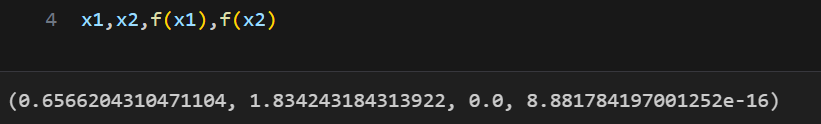
\includegraphics[width=0.5\textwidth]{第三问输出实例.png}
    \caption{第三问输出实例}
    \label{fig:第三问输出实例}
\end{figure}
如图\ref{fig:第三问输出实例}所示。

\section{题目2:Search for the minimum of the function $h\left(x,y\right)=\sin(x+y)+\cos (x+2y)$ in the whole space}
\subsection{程序描述}
g(x,y)在x轴和y轴上均具有周期$2\pi$,因此只需要计算$(x,y)\in (0,2\pi]^2$范围内的最小值即可,其就为全局最小值。可以直接解析算出,其落在该范围内的全局最小值点在$(0,1.5\pi)$处得到。

先通过将该区域分为1000个小方格,分别计算其函数值画出函数大致图像(如图\ref{fig:第二题目函数图像}所示)并找到最小值大概位置。

然后将该点记为梯度下降的起始点$(x_0,y_0)$借助最速梯度下降算法(算法\ref{Steepest-descent method})将结果精确到小数点后4位数
\begin{figure}
    \centering
    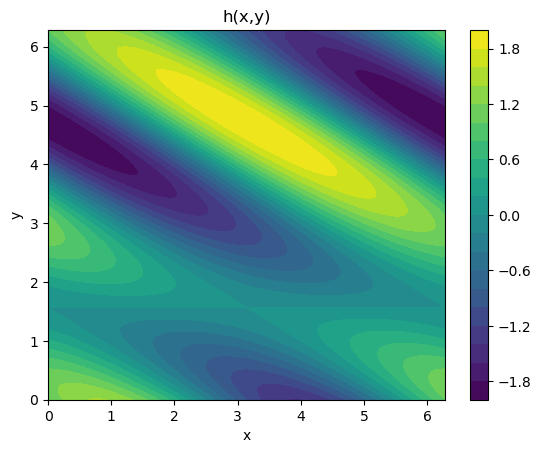
\includegraphics[width=0.5\textwidth]{第二题目函数图像.png}
    \caption{第二题目函数图像}
    \label{fig:第二题目函数图像}
\end{figure}

\subsection{伪代码}
\begin{breakablealgorithm}
    \caption{Steepest-descent method}
    \label{Steepest-descent method}
    \begin{algorithmic}
        \Require $h(x,y):function((float,float)\to float) \quad (x_0,y_0),a,epsilon:float $
        \Ensure $(x_{min},y_{min}),h_{min}$
        \State $x = x_0 y =y_0$
        \While{$||\nabla h||^2 < \epsilon$}
        \State $x\gets x-a\cdot\frac{\nabla h}{||\nabla h||} \qquad y\gets y-a\cdot\frac{\nabla h}{||\nabla h||}$
        \EndWhile
    \State \Return $x_{min} = x \quad  y_{min} = y \quad h_{min} = h(x,y)$
    \end{algorithmic}
\end{breakablealgorithm}

\subsection{输出实例}
首先,直接进行遍历求最小值,得到结果如图\ref{fig:第二题直接遍历输出结果}所示,与解析解$1.5\pi \approx 4.71238898$对比精度只有小数点后2位,借助最速下降算法(算法\ref{Steepest-descent method})进一步求解后得到结果如图\ref{fig:第二题输出实例},精度提升至小数点后4位。
\begin{figure}
    \centering
    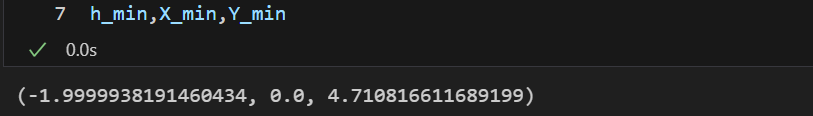
\includegraphics[width=0.5\textwidth]{第二题直接遍历输出结果.png}
    \caption{第二题直接遍历输出结果}
    \label{fig:第二题直接遍历输出结果}
\end{figure}

\begin{figure}
    \centering
    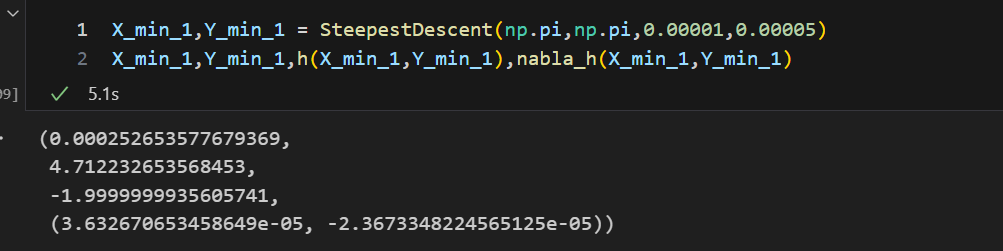
\includegraphics[width=0.5\textwidth]{第二题输出实例.png}
    \caption{第二题输出实例}
    \label{fig:第二题输出实例}
\end{figure}

\section{第四题:解电子在特定有限深方势阱的束缚态波函数}
对电子的定态薛定谔方程
\begin{equation}
    -\frac{\hbar^{2}}{2m}\frac{d^{2}\psi\left(x\right)}{dx^{2}}+V(x)\psi(x)=E\psi(x)
\end{equation}
其中$V(x)$满足:
\begin{equation}
    V(x)=\begin{cases}V_0&\quad x \le -a\\0&\quad-a <x <a\\V_0&\quad x \ge a\end{cases}
\end{equation}
则其解可以被写为
\begin{equation}
\label{波函数形式}
    \begin{aligned}
&\psi_{\mathrm{I}}=Ce^{\beta x} \beta=\sqrt{2m(V_{0}-E)}/\hbar  \\
&\psi_{\mathrm{II}}=A\sin\alpha x+B\cos\alpha x\quad\alpha=\sqrt{2mE}/\hbar \\
&\psi_{\mathrm{III}}=Fe^{-\beta x}
\end{aligned}
\end{equation}
借助边界条件和群论,可以得到其解可以被分为两种
\begin{itemize}
    \item 偶态:$A=0 \quad B\cos\alpha a=Ce^{-\beta a} \quad C=F$
    \item 奇态:$B=0 \quad -A\cos\alpha a=Ce^{-\beta a} \quad C=-F$
\end{itemize}
因此对偶态和奇态,只需要分别解满足方程
\begin{equation}
\begin{aligned}
    f_{even}(\mathrm{E})&=\alpha\sin\alpha a-\beta\cos\alpha a=0 \\
    f_{odd}(\mathrm{E})&=\alpha\sin\alpha a+\beta\cos\alpha a=0
\end{aligned}
\end{equation}
分别画出其大致函数图像如图\ref{fig:第三题待解方程大致图像}所示,能量最低的三个本征态中有两个是偶数态(0.2到0.3之间)和(1.5到1.6之间),一个为奇数态(0.8到0.9之间),考虑最后一个根距离边界$1.6\times 10^{-18}J$很近,外加函数导数情况难以判断,用差分法求导数后借助混合法(算法\ref{Newton Bisection Hybrid})求其根,再带回公式\ref{波函数形式}得到相应波函数。
\begin{figure}
    \centering
    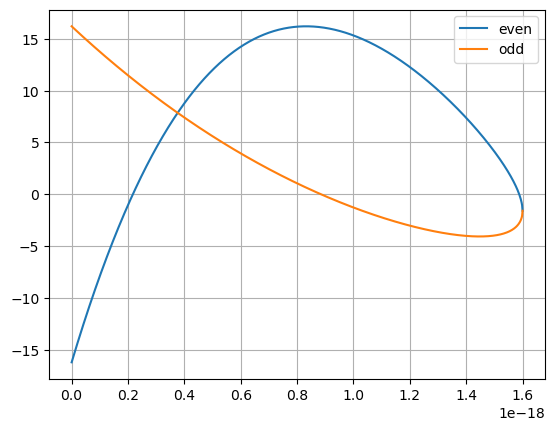
\includegraphics[width=0.5\textwidth]{第三题待解方程大致图像.png}
    \caption{第三题待解方程大致图像}
    \label{fig:第三题待解方程大致图像}
\end{figure}

\subsection{输出示例}
求得三个最低的本征能量以焦耳J为单位和以电子伏特eV分别如图\ref{fig:三个最低本征能量}所示,
\begin{figure}
    \centering
    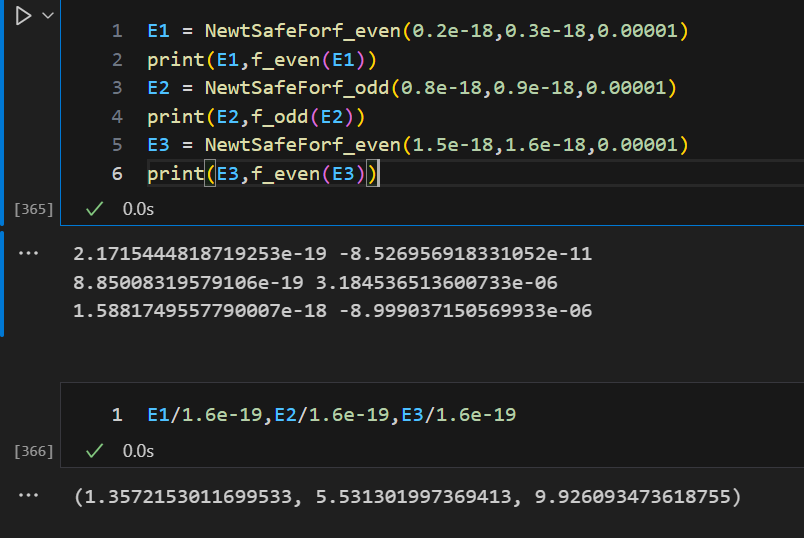
\includegraphics[width=0.5\textwidth]{三个最低本征能量.png}
    \caption{三个最低本征能量}
    \label{fig:三个最低本征能量}
\end{figure}
得到归一化前的波函数$\psi$图像如图\ref{fig:波函数(未归一化)图像},对应概率密度图像$|\Psi|^2$如图\ref{fig:概率密度函数图像}所示。
\begin{figure}
    \centering
    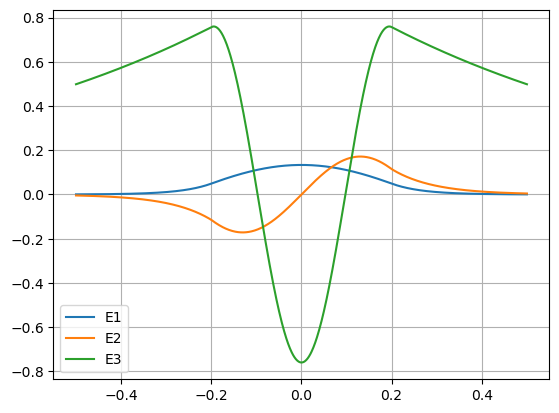
\includegraphics[width=0.5\textwidth]{波函数(未归一化)图像.png}
    \caption{波函数(未归一化)图像}
    \label{fig:波函数(未归一化)图像}
\end{figure}
\begin{figure}
    \centering
    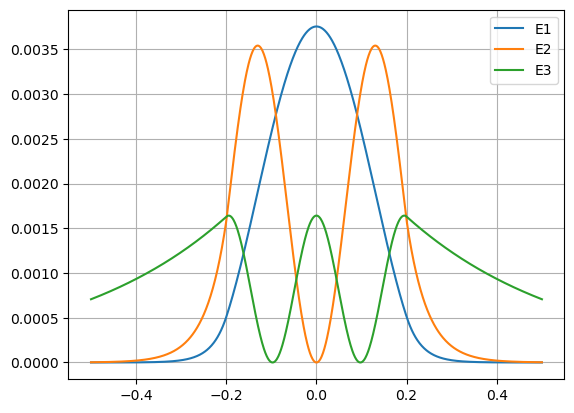
\includegraphics[width=0.5\textwidth]{概率密度函数图像.png}
    \caption{概率密度函数图像}
    \label{fig:概率密度函数图像}
\end{figure}
\end{document}